%%%%%%%%%%%%%%%%%%%%%%%%%%%%%%%%%%%%%%%%%
% Masters/Doctoral Thesis 
% LaTeX Template
% Version 1.43 (17/5/14)
%
% This template has been downloaded from:
% http://www.LaTeXTemplates.com
%
% Original authors:
% Steven Gunn 
% http://users.ecs.soton.ac.uk/srg/softwaretools/document/templates/
% and
% Sunil Patel
% http://www.sunilpatel.co.uk/thesis-template/
%
% License:
% CC BY-NC-SA 3.0 (http://creativecommons.org/licenses/by-nc-sa/3.0/)
%
% Note:
% Make sure to edit document variables in the Thesis.cls file
%
%%%%%%%%%%%%%%%%%%%%%%%%%%%%%%%%%%%%%%%%%

%----------------------------------------------------------------------------------------
%	PACKAGES AND OTHER DOCUMENT CONFIGURATIONS
%----------------------------------------------------------------------------------------

\documentclass[12pt, oneside]{Thesis} % The default font size and one-sided printing (no margin offsets)
%\usepackage[margin=1in]{geometry}
\graphicspath{{Pictures/}} % Specifies the directory where pictures are stored
\usepackage{times}
\usepackage{graphicx} % Required for including pictures
\usepackage{amsmath}
\usepackage[protrusion=true,expansion=true]{microtype} % Better typography
%\usepackage[square, numbers, comma, sort&compress]{natbib} % Use the natbib reference package - read up on this to edit the reference style; if you want text (e.g. Smith et al., 2012) for the in-text references (instead of numbers), remove 'numbers' 
\usepackage[natbibapa,unnumberedbib]{apacite} 
\hypersetup{urlcolor=blue, colorlinks=true} % Colors hyperlinks in blue - change to black if annoying
\title{\ttitle} % Defines the thesis title - don't touch this

\begin{document}

\frontmatter % Use roman page numbering style (i, ii, iii, iv...) for the pre-content pages

\setstretch{1.3} % Line spacing of 1.3

% Define the page headers using the FancyHdr package and set up for one-sided printing
\fancyhead{} % Clears all page headers and footers
\rhead{\thepage} % Sets the right side header to show the page number
\lhead{} % Clears the left side page header

\pagestyle{fancy} % Finally, use the "fancy" page style to implement the FancyHdr headers

\newcommand{\HRule}{\rule{\linewidth}{0.5mm}} % New command to make the lines in the title page

% PDF meta-data
\hypersetup{pdftitle={\ttitle}}
\hypersetup{pdfsubject=\subjectname}
\hypersetup{pdfauthor=\authornames}
\hypersetup{pdfkeywords=\keywordnames}

%----------------------------------------------------------------------------------------
%	TITLE PAGE
%----------------------------------------------------------------------------------------

\begin{titlepage}
\begin{center}

\textsc{\LARGE \university}\\[1.5cm] % University name
\textsc{\Large Masteral Thesis Proposal}\\[0.5cm] % Thesis type

\HRule \\[0.4cm] % Horizontal line
{\huge \bfseries \ttitle}\\[0.4cm] % Thesis title
\HRule \\[1.5cm] % Horizontal line
 
\begin{minipage}{0.4\textwidth}
\begin{flushleft} \large
\emph{Author:}\\
{\authornames} % Author name - remove the \href bracket to remove the link
\end{flushleft}
\end{minipage}
\begin{minipage}{0.4\textwidth}
\begin{flushright} \large
\emph{Adviser:} \\
{\supname} % Supervisor name - remove the \href bracket to remove the link  
\end{flushright}
\end{minipage}\\[3cm]
 
\large \textit{A thesis submitted in fulfilment of the requirements\\ for the degree of \degreename}\\[0.3cm] % University requirement text
\textit{in}\\[0.4cm]
\deptname\\[2cm] % Research group name and department name
 
{\large \today}\\[4cm] % Date
%\includegraphics{Logo} % University/department logo - uncomment to place it
 
\vfill
\end{center}

\end{titlepage}

%----------------------------------------------------------------------------------------
%	DECLARATION PAGE
%	Your institution may give you a different text to place here
%----------------------------------------------------------------------------------------

\Declaration{

\addtocontents{toc}{\vspace{1em}} % Add a gap in the Contents, for aesthetics

I, \authornames, declare that this thesis titled, '\ttitle' and the work presented in it are my own. I confirm that:

\begin{itemize} 
\item[\tiny{$\blacksquare$}] This work was done wholly or mainly while in candidature for a research degree at this University.
\item[\tiny{$\blacksquare$}] Where any part of this thesis has previously been submitted for a degree or any other qualification at this University or any other institution, this has been clearly stated.
\item[\tiny{$\blacksquare$}] Where I have consulted the published work of others, this is always clearly attributed.
\item[\tiny{$\blacksquare$}] Where I have quoted from the work of others, the source is always given. With the exception of such quotations, this thesis is entirely my own work.
\item[\tiny{$\blacksquare$}] I have acknowledged all main sources of help.
\item[\tiny{$\blacksquare$}] Where the thesis is based on work done by myself jointly with others, I have made clear exactly what was done by others and what I have contributed myself.\\
\end{itemize}
 
Signed:\\
\rule[1em]{25em}{0.5pt} % This prints a line for the signature
 
Date:\\
\rule[1em]{25em}{0.5pt} % This prints a line to write the date
}

\clearpage % Start a new page

%----------------------------------------------------------------------------------------
%	QUOTATION PAGE
%----------------------------------------------------------------------------------------

\pagestyle{empty} % No headers or footers for the following pages

\null\vfill % Add some space to move the quote down the page a bit

\textit{``Thanks to my solid academic training, today I can write hundreds of words on virtually any topic without possessing a shred of information, which is how I got a good job in journalism."}

\begin{flushright}
Dave Barry
\end{flushright}

\vfill\vfill\vfill\vfill\vfill\vfill\null % Add some space at the bottom to position the quote just right

\clearpage % Start a new page

%----------------------------------------------------------------------------------------
%	ABSTRACT PAGE
%----------------------------------------------------------------------------------------

\addtotoc{Abstract} % Add the "Abstract" page entry to the Contents

\abstract{\addtocontents{toc}{\vspace{1em}} % Add a gap in the Contents, for aesthetics

The Thesis Abstract is written here (and usually kept to just this page). The page is kept centered vertically so can expand into the blank space above the title too\ldots
}

\clearpage % Start a new page

%----------------------------------------------------------------------------------------
%	ACKNOWLEDGEMENTS
%----------------------------------------------------------------------------------------

\setstretch{1.3} % Reset the line-spacing to 1.3 for body text (if it has changed)

\acknowledgements{\addtocontents{toc}{\vspace{1em}} % Add a gap in the Contents, for aesthetics

The acknowledgments and the people to thank go here, don't forget to include your project advisor\ldots
}
\clearpage % Start a new page

%----------------------------------------------------------------------------------------
%	LIST OF CONTENTS/FIGURES/TABLES PAGES
%----------------------------------------------------------------------------------------

\pagestyle{fancy} % The page style headers have been "empty" all this time, now use the "fancy" headers as defined before to bring them back

\lhead{\emph{Table of Contents}} % Set the left side page header to "Contents"
\tableofcontents % Write out the Table of Contents

\lhead{\emph{List of Figures}} % Set the left side page header to "List of Figures"
\listoffigures % Write out the List of Figures

\lhead{\emph{List of Tables}} % Set the left side page header to "List of Tables"
\listoftables % Write out the List of Tables

%----------------------------------------------------------------------------------------
%	ABBREVIATIONS
%----------------------------------------------------------------------------------------

\clearpage % Start a new page

\setstretch{1.5} % Set the line spacing to 1.5, this makes the following tables easier to read

\lhead{\emph{Abbreviations}} % Set the left side page header to "Abbreviations"
\listofsymbols{ll} % Include a list of Abbreviations (a table of two columns)
{
\textbf{LAH} & \textbf{L}ist \textbf{A}bbreviations \textbf{H}ere \\
%\textbf{Acronym} & \textbf{W}hat (it) \textbf{S}tands \textbf{F}or \\
}

%----------------------------------------------------------------------------------------
%	PHYSICAL CONSTANTS/OTHER DEFINITIONS
%----------------------------------------------------------------------------------------

\clearpage % Start a new page

\lhead{\emph{Physical Constants}} % Set the left side page header to "Physical Constants"

\listofconstants{lrcl} % Include a list of Physical Constants (a four column table)
{
Speed of Light & $c$ & $=$ & $2.997\ 924\ 58\times10^{8}\ \mbox{ms}^{-\mbox{s}}$ (exact)\\
% Constant Name & Symbol & = & Constant Value (with units) \\
}

%----------------------------------------------------------------------------------------
%	SYMBOLS
%----------------------------------------------------------------------------------------

\clearpage % Start a new page

\lhead{\emph{Symbols}} % Set the left side page header to "Symbols"

\listofnomenclature{lll} % Include a list of Symbols (a three column table)
{
$a$ & distance & m \\
$P$ & power & W (Js$^{-1}$) \\
% Symbol & Name & Unit \\

& & \\ % Gap to separate the Roman symbols from the Greek

$\omega$ & angular frequency & rads$^{-1}$ \\
% Symbol & Name & Unit \\
}

%----------------------------------------------------------------------------------------
%	DEDICATION
%----------------------------------------------------------------------------------------

\setstretch{1.3} % Return the line spacing back to 1.3

\pagestyle{empty} % Page style needs to be empty for this page

\dedicatory{For/Dedicated to/To my\ldots} % Dedication text

\addtocontents{toc}{\vspace{2em}} % Add a gap in the Contents, for aesthetics

%----------------------------------------------------------------------------------------
%	THESIS CONTENT - CHAPTERS
%----------------------------------------------------------------------------------------

\mainmatter % Begin numeric (1,2,3...) page numbering

\pagestyle{fancy} % Return the page headers back to the "fancy" style

% Include the chapters of the thesis as separate files from the Chapters folder
% Uncomment the lines as you write the chapters

% Chapter 1

\chapter{INTRODUCTION} % Main chapter title

\label{Chapter1} % For referencing the chapter elsewhere, use \ref{Chapter1} 

\lhead{Chapter 1. \emph{Introduction}} % This is for the header on each page - perhaps a shortened title

%----------------------------------------------------------------------------------------

\section{Background of the Study}
The advent of ultra high resolution television screens and monitors have been 
Common video sources do not use the full capability of most high-resolution televisions of today
Super-resolution is the process of rendering or recovering a larger image or video given some low-resolution source \citep{Dong2014}
Super-resolution finds its applications in diverse fields of study. Examples include video surveillance, in \cite{Caner2003} and \cite{Zhang2010},  medical imaging [3,4], and satellite imaging [5–7], have gained significant interests in consumer electronics, academia, and industries (temporary citation)  \citep{Cheng2013}
Image super-resolution methods that use a set of LR images construct an HR image by exploring the spatial correlations in that set \citep{Cheng2013}.
\cite{Ishizaka2013} noted that "high quality SR that can be used for enterprise systems such like broadcasting and video surveillance is very compute intensive. Realtimeness is recognized as important threshold to use SR for a variety of systems. However, for example, it is several times slower than realtime to convert SD to HD by using a commodity server."

Video super-resolution is a difficult task, especially when given severe time constraints (near real-time)
Today's state-of-the-art video super-resolution methods run on a GPU (high cost, high wattage)
Current solutions also have unstable frame rates.
FPGAs are known to have high performance-per-watt ratios.

%----------------------------------------------------------------------------------------

\section{Statement of the Problem}

We are then confronted by the problem of finding a video super-resolution system that uses
a fast algorithm to generate high-quality hi-resolution videos from a low-resolution source 
while maintaining a relatively small power footprint.


%----------------------------------------------------------------------------------------

\section{Objectives of the Study}

\subsection{General Objective}

This study aims to come up with a new video super-resolution algorithm and implement this for use on an FPGA (field programmable gate array).


\subsection{Specific Objectives}

Specifically, the study aims on improving on the state-of-the-art video super-resolution algorithm in terms of PSNR (peak signal-to-noise ratio) and processing time
Determine the FPGA best suited for the purpose of video super-resolution, considering processing resources and power consumption
Profile the video super-resolution algorithm to determine performance bottlenecks
Exploit parallelizable steps in the algorithm to further enhance suitability on an FPGA


%----------------------------------------------------------------------------------------

\section{Scope and Limitations of the Study}

\begin{itemize}
\item Near real-time 
\end{itemize}

Since previous studies (cite something) have shown that clear upscaling is practical only at a factor of 4, 
it has been decided that this study should concern itself with x4 upscaling only.


%\subsection{Using US Letter Paper}
%
%The paper size used in the template is A4, which is a common -- if not standard -- size in Europe. If you are using this thesis template elsewhere and particularly in the United States, then you may have to change the A4 paper size to the US Letter size. Unfortunately, this is not as simple as replacing instances of `\texttt{a4paper}' with `\texttt{letterpaper}'.
%
%This is because the final PDF file is created directly from the \LaTeX{} source using a program called `\texttt{pdfTeX}' and in certain conditions, paper size commands are ignored and all documents are created with the paper size set to the size stated in the configuration file for pdfTeX (called `\texttt{pdftex.cfg}').
%
%What needs to be done is to change the paper size in the configuration file for \texttt{pdfTeX} to reflect the letter size. There is an excellent tutorial on how to do this here: \\
%\href{http://www.physics.wm.edu/~norman/latexhints/pdf_papersize.html}{\texttt{http://www.physics.wm.edu/$\sim$norman/latexhints/pdf\_papersize.html}}
%
%It may be sufficient just to replace the dimensions of the A4 paper size with the US Letter size in the \texttt{pdftex.cfg} file. Due to the differences in the paper size, the resulting margins may be different to what you like or require (as it is common for Institutions to dictate certain margin sizes). If this is the case, then the margin sizes can be tweaked by opening up the \texttt{Thesis.cls} file and searching for the line beginning with, `$\backslash$\texttt{setmarginsrb}' (not very far down from the top), there you will see the margins specified. Simply change those values to what you need (or what looks good) and save. Now your document should be set up for US Letter paper size with suitable margins.

%\subsection{References}

%The `\texttt{natbib}' package is used to format the bibliography and inserts references such as this one \citep{Reference3}. The options used in the `\texttt{Thesis.tex}' file mean that the references are listed in numerical order as they appear in the text. Multiple references are rearranged in numerical order (e.g. \citep{Reference2, Reference1}) and multiple, sequential references become reformatted to a reference range (e.g. \citep{Reference2, Reference1, Reference3}). This is done automatically for you. To see how you use references, have a look at the `\texttt{Chapter1.tex}' source file. Many reference managers allow you to simply drag the reference into the document as you type.
%
%Scientific references should come \emph{before} the punctuation mark if there is one (such as a comma or period). The same goes for footnotes\footnote{Such as this footnote, here down at the bottom of the page.}. You can change this but the most important thing is to keep the convention consistent throughout the thesis. Footnotes themselves should be full, descriptive sentences (beginning with a capital letter and ending with a full stop).
%
%To see how \LaTeX{} typesets the bibliography, have a look at the very end of this document (or just click on the reference number links).



% Chapter 2

\chapter{REVIEW OF RELATED LITERATURE} % Main chapter title

\label{Chapter2} % Change X to a consecutive number; for referencing this chapter elsewhere, use \ref{ChapterX}

\lhead{Chapter 2. \emph{Review of Related Literature}} % Change X to a consecutive number; this is for the header on each page - perhaps a shortened title

%----------------------------------------------------------------------------------------
%	SECTION 1
%----------------------------------------------------------------------------------------

\section{Image Super-resolution}

Still-image super-resolution (SR) is the reconstruction of a high-resolution (HR) image given one, or a set of, low-resolution (HR) images. 
Super-resolution began as the problem of image restoration from a noisy signal \citep{Helstrom1967}.
The first known work that directly tackled SR is that of \cite{tsai1984multiframe}. 
Traditionally, super-resolution of images is performed with several observed LR images. This is done in order to remove artifacts introduced by the low-resolution camera sensor \citep{Yang2010a}. 
There is another approach which involves only a single observation or image.
The limited set of data severely limits the quality obtainable, thus 
the SR problem becomes ill-posed \citep{Yang2010a}.

Super-resolution is necessary in the following fields of interest \citep{Yang2010a}:
\begin{itemize}
	\item Surveillance video: 
	\item Satellite imaging:
	\item Medical imaging: In \cite{Malczewski2008}, multi-frame SR is accomplished by taking advantage of small spatial shifts in the LR image set.
	\item Video upscaling: This is the main premise of the present study, as with the rest of the papers cited in this chapter.
\end{itemize}

\subsection{Image Quality Assessment (IQA)}
Quantification of quality is a prerequisite in the improvement of the SR algorithm to be developed.
Currently, there are two primary measures of output image quality in SR, namely, the Peak Signal-to-Noise Ratio (PSNR) and the Structural Similarity Index Measure (SSIM). 
The choice of PSNR or SSIM is typically arbitrary, with a few informal arguments favoring one or the other \citep{Farsiu2004}.
To aid in selection of a suitable metric, an analysis of both image metrics is found in \cite{Hore2010}. 
They state that a mathematical relationship exists between the two metrics, thus making it possible to predict the PSNR from the SSIM and vice-versa. 
They only differ in their sensitivity to image degradations as introduced by noise, compression, and hardware limitations.
	
A recent addition to the list of metrics is the FSIM (Feature Similarity Index Measure) \citep{Zhang2011a}.

To the present day, super-resolution remains an active area of research. 
The following sections present various approaches to SR that rely on several different models.

%---------------
\subsection{Image Observation Model}

Several factors affect the output of a digital system, including finite aperture size and finite sensor size \citep{Yang2010a}. 

\subsection{Frequency Domain}
The first SR paper as authored by \cite{tsai1984multiframe} describes the SR process in the frequency domain. 
Their algorithm takes advantage of the shift and aliasing properties of the continuous and discrete Fourier transforms, given a set of multiple shifted low resolution images. 
A few extensions have been proposed, such as 
\citep{Yang2010a}

\subsection{Interpolation-restoration}

\citep{Yang2010}

\subsection{Statistical Methods}
Hello
\citep{Yang2010a}

\subsection{Set-theoretic Methods}
Hello
\citep{Yang2010a}

\subsection{Methods Based on Sparse Representations}
The relative absence of data in the low resolution patches makes it reasonable to consider the LR patch space as a sparse representation of the HR patch space.

\cite{Zeyde2012} proposed an algorithm that uses the Sparseland model previously developed by \cite{Elad2006}.
\subsection{Dictionary Learning Methods}
Digital signal data take up too much storage space, but most of this space does not account for the most significant components of the signal it represents.
Compression and alternative representations are therefore required to reduce storage size while preserving fidelity.
The use of orthogonal and bi-orthogonal bases in 
Dictionary learning is the process of training a set of mutually orthogonal basis vectors in order to create a dictionary matrix. 
This matrix can then model any signal as a combination of its columns, better known as "atoms". (citation here)

\cite{Wright2010} jointly trained a dictionary for low resolution and another for high resolution patches to enforce sparse representation similarity for both patch spaces. Their approach is also robust to noise, as it uses local sparse modeling.
\cite{Yang2012} similarly stressed the importance of learning two coupled dictionaries, (observation dictionary and latent dictionary). However, the difference in their methods is that they used a coupled dictionary learning method for single-image SR. 	


\subsection{Computational Intelligence Methods}
So far, the previous methods mentioned all have solid mathematical foundations.
However, it has been found out (citation here) that a great number of real-world problems cannot be modeled into well-posed mathematical problems, including super-resolution.
A class of algorithms under "computational intelligence" rely on mimicking natural systems to model and solve such kinds of problems.

\cite{Dong2014} used a deep convolutional neural network in order to 


\section{Challenges in Image SR}
Researchers still struggle with the following challenges, despite years of research.
\begin{itemize}
	\item Image Registration
	\item Computation Efficiency
	\item 
\end{itemize}
\subsection{Image Registration}
Image registration is the process of mapping two images both spatially and with respect to intensity \citep{Brown1992}. It is a computationally-intensive task \citep{Yang2010a}
%According to (cite here), image registration is required for the following purposes
\begin{itemize}
	\item Integrating information taken from different sensors
	\item finding changes in images taken at different times or under different conditions
	\item Inferring three dimensional information from images in which either the camera or the objects in the scene have moved
	\item Model-based object recognition
\end{itemize}

\subsection{Edge preservation}
It is typical in SR algorithms to lose details or edges in the output image/video. 
SR techniques for edge preservation have therefore been proposed. 
\cite{Vishnukumar2014} uses self-examples.
%----------------------------------------------------------------------------------------
%	SECTION 2
%----------------------------------------------------------------------------------------

\section{Video super-resolution}

Video super-resolution is the extension of image SR to moving pictures.
An additional temporal dimension can now be factored in the SR process.
It can generally be divided into two categories: incremental and simultaneous \citep{Su2011}.
The former category is faster but less visually consistent to the human eye.
\cite{Liu2014} mentions that video SR is relatively more challenging than image SR which has been studied for decades, due to the presence of an additional temporal dimension.


\subsection{Mathematical Methods}

\cite{Liu2014} propose a Bayesian video SR system that can simultaneously estimate the motion, blur kernel, and noise level.

%-----------------------------------
%	SUBSECTION 2
%-----------------------------------

\subsection{Computational Intelligence Methods}
As in image SR, video SR is a highly nonlinear task and is amenable to processing via computational intelligence. 
For example, \cite{Cheng2013} constructed an artificial neural network that uses classifiers for video SR.

\section{High Performance Computing Platforms}
\cite{Yang2010a} suggest that high-performance hardware matters in tackling super-resolution problems. 
Typically, image SR algorithms are first developed for computer CPUs.
Modern CPUs (central processing units) of computers combine high-frequency processors with a degree of parallelism to add more processing power to algorithms.
Even so, the CPU is not enough to handle tasks such as SR in real-time.
There are several steps in the SR process that may be implemented as parallel tasks.
Following are the discussions on GPUs, manycore coprocessors, and FPGAs, three parallel platforms commonly in use today.

\subsection{Graphics Processing Units}
General-purpose computing on Graphics Processing Units
GPUs (Graphics Processing Units) have been favored in recent years for this task, as it offers high amounts of parallelism (due to its multiple cores) and compatibility with existing computer systems and programming paradigms.
\cite{Wu2011} claims 6x speedup against the same algorithm implemented on a CPU. 
\cite{Shen2014} used a real-time learning-based SR algorithm based on error feedback. 

\subsection{Manycore Coprocessors}
This class of parallel processors are based off CPU architectures but have more cores than the traditional CPU and are meant to run at a lower frequency. 
A host CPU passes the appropriate parallel instructions to the manycore coprocessor and subsequently fetches the results of the computation.
Manycore processors offer more programmability than GPUs simply by the fact that they share the same architecture as the host CPU. 
The only known product in this category is that of Intel MIC (Many Integrated Core) architecture \citep{Intel2014}.

\cite{Ishizaka2013} demonstrated a power-efficient real-time SR system that uses a virtual pipeline to improve the performance as well as the utilization of both the manycore and the host processors. 
Their set-up was able to achieve 31.5 fps, satisfying the real-time requirement.
The problem with their set up is the limited adoption of the MIC platform and the power requirement of about 170 W (check the figures).


\subsection{Field Programmable Gate Arrays (FPGAs)}
FPGAs (Field Programmable Gate Arrays) are logic devices that can be reconfigured by a designer on the field after being manufactured.
Since at the lowest level, logic circuits are inherently parallel and real-time, FPGAs offer optimization potential that cannot be realized when using instruction-based platforms such as CPUs and GPUs. FPGAs typically run at much lower frequencies than CPUs and GPUs, making them more power efficient.
Higher-end FPGAs even offer the ability to be partially dynamically reconfigured, so that even while it is running, parts of the FPGA fabric gets their design altered \citep{Dye2012}.
These factors makes FPGAs suitable for the most computationally-intensive real-time applications while conserving energy.
	
\cite{Sirowy2008} investigated the reasons why an FPGA offers high speedups over instruction-based processors such as CPU, manycore, and GPU. 
Among these are the removal of an instruction fetch step.

\subsection{Design Considerations and Strategies}
Since the SR system of this study is to be integrated into other computing systems, it is imperative to develop an embedded system, one which consumes less space on the motherboard and uses less energy.
The more power used, the more heat is generated. According to \cite{Anderson2003}, failure rates double for every 15 degree Celsius rise in temperature.
In this light, for an embedded system, the GPU and CPU are not applicable processors.
\cite{Mittal2014} considered using an "unconventional core" such as an FPGA to realize lower power-consumption in an embedded system.
\cite{Struyf2014} 



\subsubsection{Use in super-resolution applications}
The following papers prove the feasibility of an FPGA in SR applications.
\cite{Angelopoulou2009} created a real-time video SR system on an FPGA that is robust against noise.
It uses the iterative back projection algorithm. 
However, the system depends on an adaptive image sensor 
\cite{Szydzik2011} constructed a high quality SR system on an FPGA. 
They were able to achieve 2x upscaling at 25 fps while using only less than 37\% of FPGA resources of the state-of-the-art algorithm at that time.
\cite{Bowen2008} achieved 3x speedup over equivalent software (CPU) implementations.

\subsubsection{As video processors}
\cite{Roth2011} used low-cost FPGA hardware to accomplish real-time video processing tasks such as deinterlacing, alpha blending, and frame buffering.

\section{Comparison of CPU, GPU and FPGA}

\cite{Asano2009} compared the performance of the CPU, GPU and FPGA in image processing applications. 
They noted that CPUs are consistently lagging behind the GPU and FPGA, while the GPU is best for "naive computation methods" in which processing takes place on a per pixel basis.

\cite{Fowers2012} compared the performance and the energy expended by FPGAs, GPUs and multicore CPUs. 
This paper is significant to the present study since their focus is on sliding-window algorithms, which take the data on a per-block basis instead of per-pixel. This makes computation more efficient.

\section{Zynq-7000 System-on-a-chip}

 
% Chapter 3

\chapter{CONCEPTUAL FRAMEWORK} % Main chapter title

\label{Chapter3} % Change X to a consecutive number; for referencing this chapter elsewhere, use \ref{ChapterX}

\lhead{Chapter 3. \emph{Conceptual Framework}} % Change X to a consecutive number; this is for the header on each page - perhaps a shortened title

%----------------------------------------------------------------------------------------
%	SECTION 1
%----------------------------------------------------------------------------------------



%\begin{figure}[htbp]
%	\centering
%	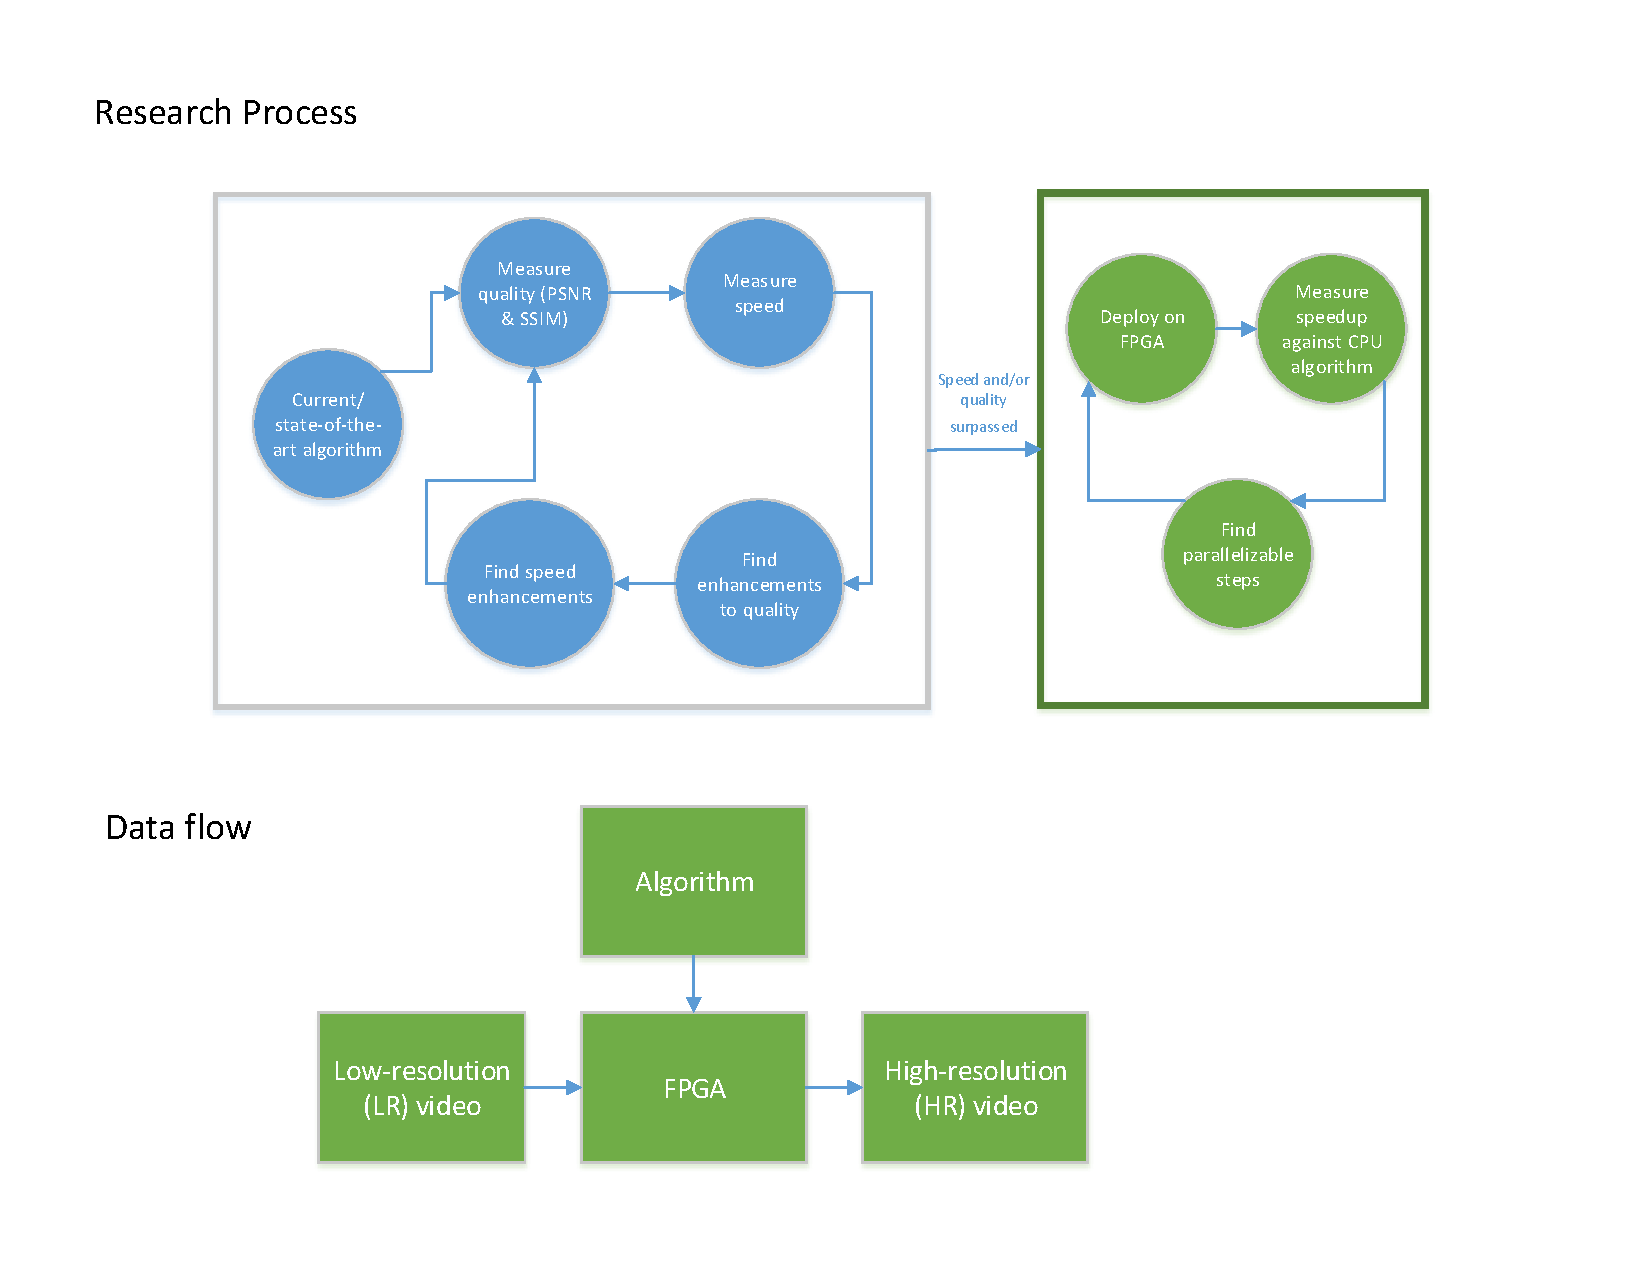
\includegraphics{Figures/framework.pdf}
%	\rule{35em}{0.2pt}
%	\caption[Conceptual Framework]{Conceptual Framework of the Study.}
%	\label{fig:Framework}
%\end{figure}



%-----------------------------------
%	SUBSECTION 1
%-----------------------------------
\section{Algorithm Framework}
% Place figure here

% Explain the framework

%-----------------------------------
%	SUBSECTION 2
%-----------------------------------

\section{Hardware Framework}
\begin{figure}
	\centering
	\includegraphics[scale=0.5]{Figures/HARDWARE_FRAMEWORK.png}
	\caption[]{Framework for Hardware Implementation.}
	\label{fig:hardframe}
\end{figure}

% Explain the framework
Figure \ref{fig:hardframe} illustrates the flow of data across the hardware devices to be used in the study.
A video source such as a camera or prerecorded file will be sent for super-resolution on the SoC, which will then display the result on the monitor in real-time.
Initially a conventional computer will serve as the development and evaluation  environment for the SR algorithm.
A revised version of the algorithm can then be sent to the SoC for further testing and fine-tuning.



%----------------------------------------------------------------------------------------
%	SECTION 2
%----------------------------------------------------------------------------------------

% Chapter 4

\chapter{METHODOLOGY} % Main chapter title

\label{Chapter4} % Change X to a consecutive number; for referencing this chapter elsewhere, use \ref{ChapterX}

\lhead{Chapter 4. \emph{METHODOLOGY}} % Change X to a consecutive number; this is for the header on each page - perhaps a shortened title

%----------------------------------------------------------------------------------------
%	SECTION 1
%----------------------------------------------------------------------------------------

\section{Image Super-resolution}

Lorem ipsum dolor sit amet, consectetur adipiscing elit. Aliquam ultricies lacinia euismod. Nam tempus risus in dolor rhoncus in interdum enim tincidunt. Donec vel nunc neque. In condimentum ullamcorper quam non consequat. Fusce sagittis tempor feugiat. Fusce magna erat, molestie eu convallis ut, tempus sed arcu. Quisque molestie, ante a tincidunt ullamcorper, sapien enim dignissim lacus, in semper nibh erat lobortis purus. Integer dapibus ligula ac risus convallis pellentesque.

%-----------------------------------
%	SUBSECTION 1
%-----------------------------------
\subsection{Mathematical Methods}

Nunc posuere quam at lectus tristique eu ultrices augue venenatis. Vestibulum ante ipsum primis in faucibus orci luctus et ultrices posuere cubilia Curae; Aliquam erat volutpat. Vivamus sodales tortor eget quam adipiscing in vulputate ante ullamcorper. Sed eros ante, lacinia et sollicitudin et, aliquam sit amet augue. In hac habitasse platea dictumst.

%-----------------------------------
%	SUBSECTION 2
%-----------------------------------

\subsection{Computational Intelligence Methods}
Morbi rutrum odio eget arcu adipiscing sodales. Aenean et purus a est pulvinar pellentesque. Cras in elit neque, quis varius elit. Phasellus fringilla, nibh eu tempus venenatis, dolor elit posuere quam, quis adipiscing urna leo nec orci. Sed nec nulla auctor odio aliquet consequat. Ut nec nulla in ante ullamcorper aliquam at sed dolor. Phasellus fermentum magna in augue gravida cursus. Cras sed pretium lorem. Pellentesque eget ornare odio. Proin accumsan, massa viverra cursus pharetra, ipsum nisi lobortis velit, a malesuada dolor lorem eu neque.

%----------------------------------------------------------------------------------------
%	SECTION 2
%----------------------------------------------------------------------------------------

\section{Video super-resolution}

Sed ullamcorper quam eu nisl interdum at interdum enim egestas. Aliquam placerat justo sed lectus lobortis ut porta nisl porttitor. Vestibulum mi dolor, lacinia molestie gravida at, tempus vitae ligula. Donec eget quam sapien, in viverra eros. Donec pellentesque justo a massa fringilla non vestibulum metus vestibulum. Vestibulum in orci quis felis tempor lacinia. Vivamus ornare ultrices facilisis. Ut hendrerit volutpat vulputate. Morbi condimentum venenatis augue, id porta ipsum vulputate in. Curabitur luctus tempus justo. Vestibulum risus lectus, adipiscing nec condimentum quis, condimentum nec nisl. Aliquam dictum sagittis velit sed iaculis. Morbi tristique augue sit amet nulla pulvinar id facilisis ligula mollis. Nam elit libero, tincidunt ut aliquam at, molestie in quam. Aenean rhoncus vehicula hendrerit.

\subsection{Mathematical Methods}

Nunc posuere quam at lectus tristique eu ultrices augue venenatis. Vestibulum ante ipsum primis in faucibus orci luctus et ultrices posuere cubilia Curae; Aliquam erat volutpat. Vivamus sodales tortor eget quam adipiscing in vulputate ante ullamcorper. Sed eros ante, lacinia et sollicitudin et, aliquam sit amet augue. In hac habitasse platea dictumst.

%-----------------------------------
%	SUBSECTION 2
%-----------------------------------

\subsection{Computational Intelligence Methods}
Morbi rutrum odio eget arcu adipiscing sodales. Aenean et purus a est pulvinar pellentesque. Cras in elit neque, quis varius elit. Phasellus fringilla, nibh eu tempus venenatis, dolor elit posuere quam, quis adipiscing urna leo nec orci. Sed nec nulla auctor odio aliquet consequat. Ut nec nulla in ante ullamcorper aliquam at sed dolor. Phasellus fermentum magna in augue gravida cursus. Cras sed pretium lorem. Pellentesque eget ornare odio. Proin accumsan, massa viverra cursus pharetra, ipsum nisi lobortis velit, a malesuada dolor lorem eu neque.

\section{Field Programmable Gate Arrays (FPGAs)}

Lorem ipsum dolor sit amet, consectetur adipiscing elit. Aliquam ultricies lacinia euismod. Nam tempus risus in dolor rhoncus in interdum enim tincidunt. Donec vel nunc neque. In condimentum ullamcorper quam non consequat. Fusce sagittis tempor feugiat. Fusce magna erat, molestie eu convallis ut, tempus sed arcu. Quisque molestie, ante a tincidunt ullamcorper, sapien enim dignissim lacus, in semper nibh erat lobortis purus. Integer dapibus ligula ac risus convallis pellentesque.

\subsection{Design Strategies}
Morbi rutrum odio eget arcu adipiscing sodales. Aenean et purus a est pulvinar pellentesque. Cras in elit neque, quis varius elit. Phasellus fringilla, nibh eu tempus venenatis, dolor elit posuere quam, quis adipiscing urna leo nec orci. Sed nec nulla auctor odio aliquet consequat. Ut nec nulla in ante ullamcorper aliquam at sed dolor. Phasellus fermentum magna in augue gravida cursus. Cras sed pretium lorem. Pellentesque eget ornare odio. Proin accumsan, massa viverra cursus pharetra, ipsum nisi lobortis velit, a malesuada dolor lorem eu neque.

\subsection{Use in other high performance-per-watt applications}
Morbi rutrum odio eget arcu adipiscing sodales. Aenean et purus a est pulvinar pellentesque. Cras in elit neque, quis varius elit. Phasellus fringilla, nibh eu tempus venenatis, dolor elit posuere quam, quis adipiscing urna leo nec orci. Sed nec nulla auctor odio aliquet consequat. Ut nec nulla in ante ullamcorper aliquam at sed dolor. Phasellus fermentum magna in augue gravida cursus. Cras sed pretium lorem. Pellentesque eget ornare odio. Proin accumsan, massa viverra cursus pharetra, ipsum nisi lobortis velit, a malesuada dolor lorem eu neque.

\subsection{As video processors}
Morbi rutrum odio eget arcu adipiscing sodales. Aenean et purus a est pulvinar pellentesque. Cras in elit neque, quis varius elit. Phasellus fringilla, nibh eu tempus venenatis, dolor elit posuere quam, quis adipiscing urna leo nec orci. Sed nec nulla auctor odio aliquet consequat. Ut nec nulla in ante ullamcorper aliquam at sed dolor. Phasellus fermentum magna in augue gravida cursus. Cras sed pretium lorem. Pellentesque eget ornare odio. Proin accumsan, massa viverra cursus pharetra, ipsum nisi lobortis velit, a malesuada dolor lorem eu neque. 
% Chapter 5

\chapter{SUMMARY} % Main chapter title

\label{Chapter5} % Change X to a consecutive number; for referencing this chapter elsewhere, use \ref{ChapterX}

\lhead{Chapter 5. \emph{SUMMARY}} % Change X to a consecutive number; this is for the header on each page - perhaps a shortened title

%----------------------------------------------------------------------------------------
%	SECTION 1
%----------------------------------------------------------------------------------------

In summary, the system to be developed is a reading  
%\input{Chapters/Chapter6} 
%\input{Chapters/Chapter7} 

%----------------------------------------------------------------------------------------
%	THESIS CONTENT - APPENDICES
%----------------------------------------------------------------------------------------

\addtocontents{toc}{\vspace{2em}} % Add a gap in the Contents, for aesthetics

\appendix % Cue to tell LaTeX that the following 'chapters' are Appendices

% Include the appendices of the thesis as separate files from the Appendices folder
% Uncomment the lines as you write the Appendices

% Appendix A

\chapter{Gantt Chart} % Main appendix title

\label{AppendixA} % For referencing this appendix elsewhere, use \ref{AppendixA}

\lhead{Appendix A. \emph{Gantt Chart}} % This is for the header on each page - perhaps a shortened title

% Write your Appendix content here.

% Either use MSProj Gantt Chart, or LaTeX Gantt Chart
\begin{figure*}[!ht]
	\centering
	\includegraphics[page=1,scale=0.59]{Figures/GANTT_CHART.pdf}
\end{figure*}
%\todo{Landscape Gantt Chart}
\begin{figure*}
	\centering
	\includegraphics[page=2,scale=0.59]{Figures/GANTT_CHART.pdf}
\end{figure*}
%\begin{ganttchart}{1}{12}
%	\gantttitle{2015}{12} \\
%	\gantttitlelist{1,...,12}{1} \\
%	\ganttgroup{Group 1}{1}{7} \\
%	\ganttbar{Task 1}{1}{2} \\
%	\ganttlinkedbar{Task 2}{3}{7} \ganttnewline
%	\ganttmilestone{Milestone}{7} \ganttnewline
%	\ganttbar{Final Task}{8}{12}
%	\ganttlink{elem2}{elem3}
%	\ganttlink{elem3}{elem4}
%\end{ganttchart}
% Appendix A

\chapter{Proposed Budget} % Main appendix title

\label{AppendixB} % For referencing this appendix elsewhere, use \ref{AppendixA}

\lhead{Appendix B. \emph{Proposed Budget}} % This is for the header on each page - perhaps a shortened title

% Write your Appendix content here.
% Insert LaTeX table on proposed budget here
\begin{tabular}{ | l | l | l | }
%	\centering
	\hline
	Qty & Particulars & Unit Cost \\ \hline
	1 & Digilent ZedBoard with Xilinx Zynq-7000 SoC & 15000 \\ \hline
	1 & Paper Fees & 1000 \\ \hline
	& Total & 16000 \\ \hline
\end{tabular}

%\input{Appendices/AppendixC}

\addtocontents{toc}{\vspace{2em}} % Add a gap in the Contents, for aesthetics

\backmatter

%----------------------------------------------------------------------------------------
%	BIBLIOGRAPHY
%----------------------------------------------------------------------------------------

\label{References}

\lhead{\emph{References}} % Change the page header to say "Bibliography"

%\bibliographystyle{unsrtnat} % Use the "unsrtnat" BibTeX style for formatting the Bibliography
\bibliographystyle{apacite}
\bibliography{Bibliographies/SR_image,Bibliographies/HPC_CS,Bibliographies/SR_video,Bibliographies/HPC_SR,Bibliographies/TV_Standards,Bibliographies/Img_Proc,Bibliographies/Bibliography,Bibliographies/FPGA_ImgProc,Bibliographies/FPGA} % The references (bibliography) information are stored in the file named "Bibliography.bib"

\end{document}  